% Segmentation Pipeline Diagram
% Compile with XeLaTeX or LuaLaTeX

\documentclass[tikz,border=10pt]{standalone}
\usepackage{tikz}
\usetikzlibrary{shapes.geometric, arrows.meta, positioning, fit, backgrounds, decorations.pathreplacing, patterns}

% Define colors
\definecolor{rawgray}{RGB}{158,158,158}
\definecolor{segblue}{RGB}{33,150,243}
\definecolor{featgreen}{RGB}{76,175,80}
\definecolor{classred}{RGB}{244,67,54}

\begin{document}
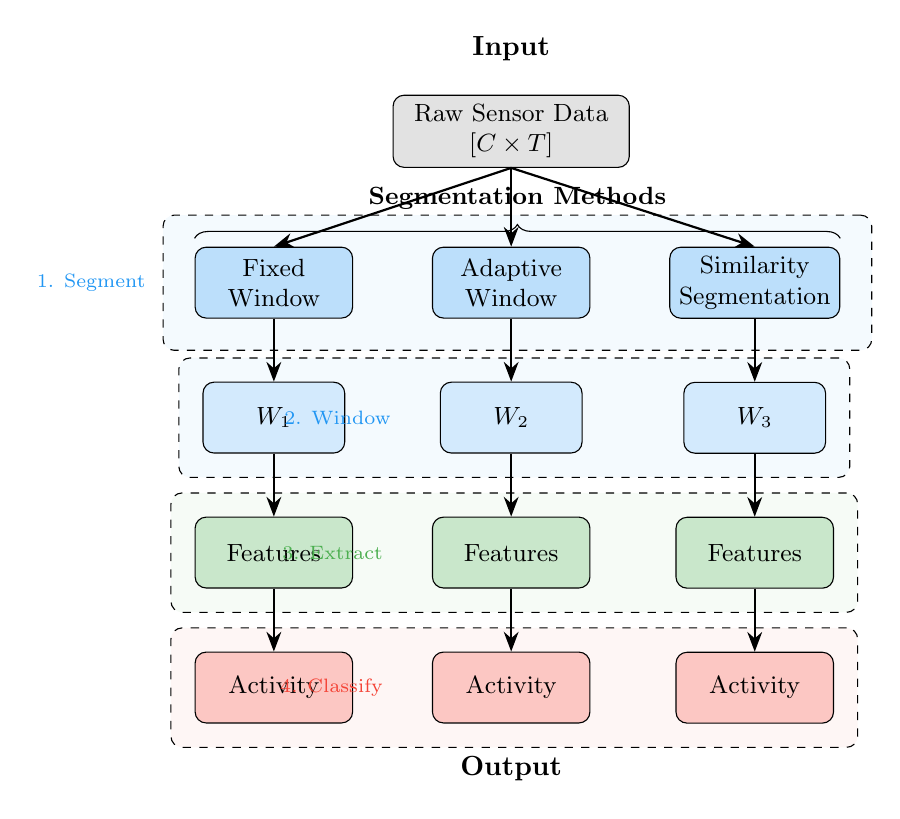
\begin{tikzpicture}[
    node distance=0.6cm,
    block/.style={rectangle, draw, fill=#1, rounded corners, minimum height=0.9cm, minimum width=2cm, align=center, font=\small},
    block/.default=white,
    arrow/.style={-{Stealth[length=2.5mm]}, thick},
    label/.style={font=\scriptsize}
]

% Raw Signal
\node[block=rawgray!30, minimum width=3cm] (raw) {Raw Sensor Data\\$[C \times T]$};

% Segmentation methods
\node[block=segblue!30, below left=1cm and 0.5cm of raw] (fixed) {Fixed\\Window};
\node[block=segblue!30, below=1cm of raw] (adaptive) {Adaptive\\Window};
\node[block=segblue!30, below right=1cm and 0.5cm of raw] (similarity) {Similarity\\Segmentation};

% Segmented windows
\node[block=segblue!20, below=0.8cm of fixed, minimum width=1.8cm] (w1) {$W_1$};
\node[block=segblue!20, below=0.8cm of adaptive, minimum width=1.8cm] (w2) {$W_2$};
\node[block=segblue!20, below=0.8cm of similarity, minimum width=1.8cm] (w3) {$W_3$};

% Feature extraction
\node[block=featgreen!30, below=0.8cm of w1] (feat1) {Features};
\node[block=featgreen!30, below=0.8cm of w2] (feat2) {Features};
\node[block=featgreen!30, below=0.8cm of w3] (feat3) {Features};

% Classification
\node[block=classred!30, below=0.8cm of feat1] (cls1) {Activity};
\node[block=classred!30, below=0.8cm of feat2] (cls2) {Activity};
\node[block=classred!30, below=0.8cm of feat3] (cls3) {Activity};

% Arrows from raw
\draw[arrow] (raw.south) -- (fixed.north);
\draw[arrow] (raw.south) -- (adaptive.north);
\draw[arrow] (raw.south) -- (similarity.north);

% Arrows through pipeline
\draw[arrow] (fixed) -- (w1);
\draw[arrow] (adaptive) -- (w2);
\draw[arrow] (similarity) -- (w3);

\draw[arrow] (w1) -- (feat1);
\draw[arrow] (w2) -- (feat2);
\draw[arrow] (w3) -- (feat3);

\draw[arrow] (feat1) -- (cls1);
\draw[arrow] (feat2) -- (cls2);
\draw[arrow] (feat3) -- (cls3);

% Labels
\node[above=0.3cm of raw, font=\bfseries] {Input};
\node[below=0.3cm of cls2, font=\bfseries] {Output};

% Brace for segmentation methods
\draw[decorate, decoration={brace, amplitude=5pt, raise=3pt}] 
    (fixed.north west) -- (similarity.north east) 
    node[midway, above=10pt, font=\small\bfseries] {Segmentation Methods};

% Dashed boxes
\begin{scope}[on background layer]
    \node[fit=(fixed)(adaptive)(similarity), draw, dashed, rounded corners, inner sep=0.4cm, fill=segblue!5] {};
    \node[fit=(w1)(w2)(w3), draw, dashed, rounded corners, inner sep=0.3cm, fill=segblue!5] {};
    \node[fit=(feat1)(feat2)(feat3), draw, dashed, rounded corners, inner sep=0.3cm, fill=featgreen!5] {};
    \node[fit=(cls1)(cls2)(cls3), draw, dashed, rounded corners, inner sep=0.3cm, fill=classred!5] {};
\end{scope}

% Pipeline stage labels
\node[left=0.5cm of fixed, label, text=segblue] {1. Segment};
\node[left=0.5cm of w2, label, text=segblue] {2. Window};
\node[left=0.5cm of feat2, label, text=featgreen] {3. Extract};
\node[left=0.5cm of cls2, label, text=classred] {4. Classify};

\end{tikzpicture}
\end{document}
